\subsection{Applicant Profile Management}

The Applicant Profile Management use case diagram consists of two primary actors: Admin and Applicant. This module handles various operations including creating accounts, updating profiles, filling up admission forms, generating and downloading the application forms, and managing edit requests.

% Diagram Input
\begin{tikzpicture}[
    node distance = 1cm and 2cm,
    usecase/.style={ellipse, draw, minimum width=4.5cm, minimum height=0.7cm, align=center, font=\small},
    link/.style={draw, thick}
]
% System Boundary
\draw[thick] (0, 0) rectangle (9, -11);
\node at (4.5, -0.5) {\textbf{Applicant Profile Management}};

% Applicant Actor (Left)
\node (applicant) at (-2, -5.5) {
    \begin{tikzpicture}[scale=0.5]
        \draw[thick] (0,1.2) circle (0.4cm); \draw[thick] (0,0.8) -- (0,-0.8);
        \draw[thick] (-0.8,0.4) -- (0.8,0.4); \draw[thick] (0,-0.8) -- (-0.5,-1.8); \draw[thick] (0,-0.8) -- (0.5,-1.8);
        \node at (0,-2.5) {\small Applicant};
    \end{tikzpicture}
};

% Admin Actor (Right)
\node (admin) at (11, -5.5) {
    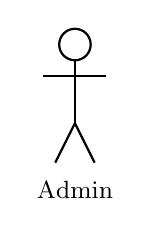
\begin{tikzpicture}[scale=0.5]
        \draw[thick] (0,1.2) circle (0.4cm); \draw[thick] (0,0.8) -- (0,-0.8);
        \draw[thick] (-0.8,0.4) -- (0.8,0.4); \draw[thick] (0,-0.8) -- (-0.5,-1.8); \draw[thick] (0,-0.8) -- (0.5,-1.8);
        \node at (0,-2.5) {\small Admin};
    \end{tikzpicture}
};

% Use Cases
\node[usecase] (uc1) at (4.5, -1.5) {Create Account};
\node[usecase] (uc2) at (4.5, -2.5) {Update Profile};
\node[usecase] (uc3) at (4.5, -3.5) {Fill-up Application Form};
\node[usecase] (uc4) at (4.5, -4.5) {Generate Application Form};
\node[usecase] (uc5) at (4.5, -5.5) {Download Application Form};
\node[usecase] (uc6) at (4.5, -6.5) {Send Edit Request};
\node[usecase] (uc7) at (4.5, -7.5) {Approve Edit Request};
\node[usecase] (uc8) at (4.5, -8.5) {Update Applicant Info};

% Connections for Applicant (Left Side)
\foreach \i in {uc1,uc2,uc3,uc4,uc5,uc6} \draw[link] (applicant) -- (\i.west);

% Connections for Admin (Right Side)
\draw[link] (admin) -- (uc7.east);
\draw[link] (admin) -- (uc8.east);

\end{tikzpicture}

\subsubsection{Create Account}
\begin{table}[!htbp]
    \centering
    \small
    \renewcommand{\arraystretch}{1.4}
    \caption{Create Account (UC-6.1)}
    \label{tab:create_account_applicant}
    \begin{tabularx}{\textwidth}{|l|X|}
        \hline
        \rowcolor[gray]{0.9} \textbf{Characteristics} & \textbf{Description} \\ \hline
        Use Case ID & UC-6.1 \\ \hline
        Use Case Name & Create Account \\ \hline
        Primary Actors & Applicant \\ \hline
        Goal & Create a new account \\ \hline
        Precondition & Must be a new user for the system \\ \hline
        Scenario & 1. Give all inputs \newline 2. Click Register button. \\ \hline
        Exception & Invalid GST Applicant ID \\ \hline
        Frequency & High \\ \hline
    \end{tabularx}
\end{table}

\subsubsection{Update Profile}
\begin{table}[!htbp]
    \centering
    \small
    \renewcommand{\arraystretch}{1.4}
    \caption{Update Profile (UC-6.2)}
    \label{tab:update_profile_applicant}
    \begin{tabularx}{\textwidth}{|l|X|}
        \hline
        \rowcolor[gray]{0.9} \textbf{Characteristics} & \textbf{Description} \\ \hline
        Use Case ID & UC-6.2 \\ \hline
        Use Case Name & Update Profile \\ \hline
        Primary Actors & Applicant \\ \hline
        Scenario & 1. Visit Dashboard \newline 2. Click Profile icon \newline 3. Select Update \newline 4. Click Update button. \\ \hline
    \end{tabularx}
\end{table}

\subsubsection{Fill-up Application Form}
\begin{table}[!htbp]
    \centering
    \small
    \renewcommand{\arraystretch}{1.4}
    \caption{Fill-up Application Form (UC-6.3)}
    \label{tab:fill_application_form}
    \begin{tabularx}{\textwidth}{|l|X|}
        \hline
        \rowcolor[gray]{0.9} \textbf{Characteristics} & \textbf{Description} \\ \hline
        Use Case ID & UC-6.3 \\ \hline
        Use Case Name & Fill-up Application Form \\ \hline
        Scenario & 1. Click Fill-up Application \newline 2. Enter Form \newline 3. Complete all 5 steps. \\ \hline
    \end{tabularx}
\end{table}

\subsubsection{Generate Application Form}
\begin{table}[!htbp]
    \centering
    \small
    \renewcommand{\arraystretch}{1.4}
    \caption{Generate Application Form (UC-6.4)}
    \label{tab:generate_application_form}
    \begin{tabularx}{\textwidth}{|l|X|}
        \hline
        \rowcolor[gray]{0.9} \textbf{Characteristics} & \textbf{Description} \\ \hline
        Use Case ID & UC-6.4 \\ \hline
        Use Case Name & Generate Application Form \\ \hline
        Scenario & 1. Visit Dashboard \newline 2. Click Generate Application Form button. \\ \hline
    \end{tabularx}
\end{table}

\subsubsection{Download Application Form}
\begin{table}[!htbp]
    \centering
    \small
    \renewcommand{\arraystretch}{1.4}
    \caption{Download Application Form (UC-6.5)}
    \label{tab:download_application_form}
    \begin{tabularx}{\textwidth}{|l|X|}
        \hline
        \rowcolor[gray]{0.9} \textbf{Characteristics} & \textbf{Description} \\ \hline
        Use Case ID & UC-6.5 \\ \hline
        Use Case Name & Download Application Form \\ \hline
        Scenario & 1. Visit Dashboard \newline 2. Click Download Application Form button. \\ \hline
    \end{tabularx}
\end{table}

\subsubsection{Send Edit Request}
\begin{table}[!htbp]
    \centering
    \small
    \renewcommand{\arraystretch}{1.4}
    \caption{Send Edit Request (UC-6.6)}
    \label{tab:send_edit_request}
    \begin{tabularx}{\textwidth}{|l|X|}
        \hline
        \rowcolor[gray]{0.9} \textbf{Characteristics} & \textbf{Description} \\ \hline
        Use Case ID & UC-6.6 \\ \hline
        Use Case Name & Send Edit Request \\ \hline
        Scenario & 1. Click Send Edit Request button. \\ \hline
    \end{tabularx}
\end{table}

\subsubsection{Approve Edit Request}
\begin{table}[!htbp]
    \centering
    \small
    \renewcommand{\arraystretch}{1.4}
    \caption{Approve Edit Request (UC-6.7)}
    \label{tab:approve_edit_request}
    \begin{tabularx}{\textwidth}{|l|X|}
        \hline
        \rowcolor[gray]{0.9} \textbf{Characteristics} & \textbf{Description} \\ \hline
        Use Case ID & UC-6.7 \\ \hline
        Use Case Name & Approve Edit Request \\ \hline
        Primary Actors & Admin \\ \hline
        Scenario & 1. Log in \newline 2. Click Edit Request \newline 3. Click Permit button. \\ \hline
    \end{tabularx}
\end{table}

\subsubsection{Update Applicant Info}
\begin{table}[!htbp]
    \centering
    \small
    \renewcommand{\arraystretch}{1.4}
    \caption{Update Applicant Information (UC-6.8)}
    \label{tab:update_applicant_info_admin}
    \begin{tabularx}{\textwidth}{|l|X|}
        \hline
        \rowcolor[gray]{0.9} \textbf{Characteristics} & \textbf{Description} \\ \hline
        Use Case ID & UC-6.8 \\ \hline
        Use Case Name & Update Applicant Information \\ \hline
        Primary Actors & Admin \\ \hline
        Scenario & 1. Log in \newline 2. Click Applicant Table \newline 3. Input values \newline 4. Click Update button. \\ \hline
    \end{tabularx}
\end{table}
\FloatBarrier